\subsection{Watchdog Module (WD) }
\label{sec:WD}

The Watchdog Module (WD) module prevents unexpected or intermittent software or hardware failures from stalling the microcontroller
indefinitely. The module expects a timer reset signal from the microcontroller withing a given period. In the absence of this
event, the watchdog circuit will reset the \mu C.

\subsubsection{Requirements}

The application runs only every second or so and the \mu C is
in power-saving mode most of the time. There are no strict timing requirements but unnecessary watchdog resets must be avoided.
This means that the watchdog circuit must be configurable for timeout periods of several seconds.
This requirement excludes many available watchdog ICs. \par

\begin{enumerate}
    \item supply voltage  \SI{3.3}{\V}.
    \item low power, low quiescent current.
    \item timeout period of several seconds.
\end{enumerate}

For my application, I choose a timeout period of roughly \SI{8}{\s}. This prevents any possible false resets due to
variations in program execution time that might be introduced by future software updates.

\subsubsection{Implementation}


\begin{table}[H]
    \centering
    \begin{threeparttable}[b]
        \begin{tabularx}{\linewidth}{
                >{\hsize=0.25\hsize}X
                >{\hsize=0.75\hsize}X
                >{\hsize=1.25\hsize}X
                >{\hsize=0.5\hsize}X
                >{\hsize=2.25\hsize}X
            }
            Id    & Desc                         & Order Code       & Package & Rationale                                         \\
            \midrule
            $U_1$ & \cite{noauthor_tps3431_2018} & TPS3431SDRBR/681 & VSON-8  & wide range of timeout values\tnote{1}             \\
            $R_p$ & 100k                         & generic          & 0603    & pull-up resistor\tnote{2}                         \\
            $C_c$ & \SI{100}{\nF}, \SI{16}{\V}   & generic          & 0603    & value for \approx \SI{8}{\s} timeout\tnote{3}     \\
            $C_b$ & \SI{100}{\nF}, \SI{16}{\V}   & generic          & 0402    & bypass cap, optional but recommended in datasheet \\
        \end{tabularx}
        \begin{tablenotes}
            \item [1] and low quiescent current, active-low open drain output suitable for Arduino dev board.
            \item [2] see \cite{noauthor_tps3431_2018}, 8.2.2.1 Calculating WDO Pullup Resistor Design 1.
            \item [3] see \cite{noauthor_tps3431_2018}, table 8-3.
        \end{tablenotes}
    \end{threeparttable}[b]
    \caption{WD Module - BOM}
    \label{table:wd1}
\end{table}

\begin{table}[H]
    \centering
    \begin{threeparttable}[b]
        \begin{tabularx}{\linewidth}{ >{\hsize=.15\hsize}X >{\hsize=1.35\hsize}X >{\hsize=1.5\hsize}X }
            \toprule
            Id & Issue                           & Potential solutions      \\
            \midrule
            1  & Make watchdog reset  persistent & add a flip-flop\tnote{1} \\
            \bottomrule
        \end{tabularx}
        \begin{tablenotes}
            \item [1] the state of the flip-flop could then be transmitted to alert a human supervisor that the circuit has malfunctioned.
        \end{tablenotes}
    \end{threeparttable}
    \caption{WD - issues}
\end{table}
\clearpage
\begin{figure}[h]
    \centering
    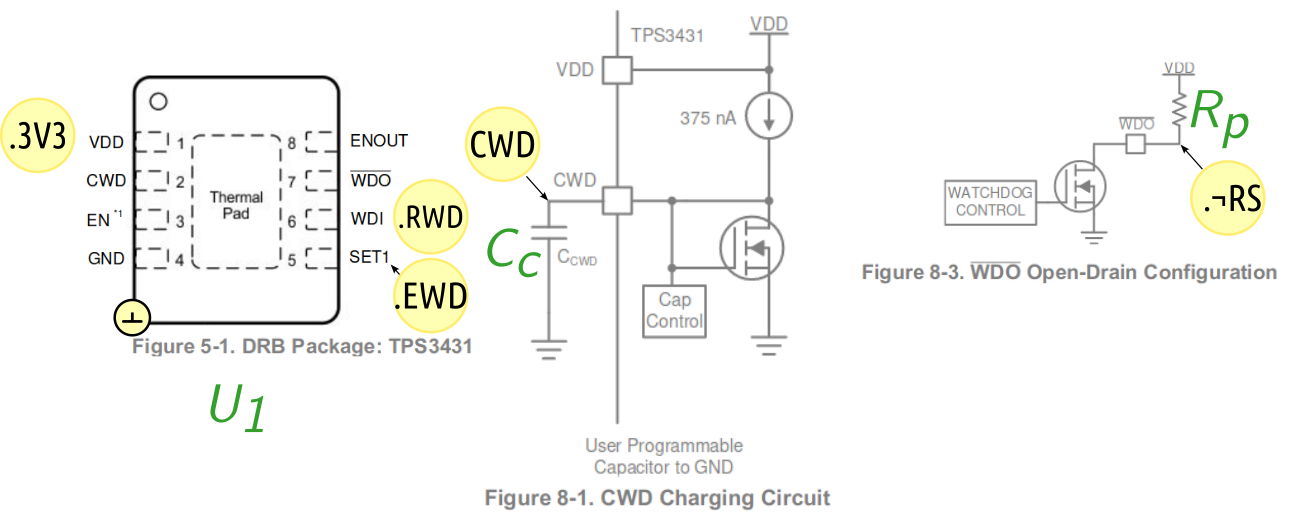
\includegraphics[width=1.0\textwidth]{MA/WD/WD}
    \caption{WD - schematic, from datasheet \cite{noauthor_tps3431_2018}}
\end{figure}

\begin{table}[H]
    \centering
    \begin{threeparttable}[b]
        \begin{tabularx}{\linewidth}{ >
                    {\hsize=.25\hsize}X >
                    {\hsize=0.5\hsize}X >
                    {\hsize=.25\hsize}X  >
                    {\hsize=.5\hsize}X >
                    {\hsize=.25\hsize}X  >
                    {\hsize=3\hsize}X
            }
                  & \multicolumn{4}{c}{pin} &                                                                                                   \\
            \cmidrule(lr){3-6}
            Id    & Net                     & Nb. & Name                        & Type            & Function                                    \\
            \midrule
            $U_1$ & .3V3                    & 1   & \texttt{VDD}                & $\leftarrow$    & power supply                                \\
            $U_1$ & CWD                     & 2   & \texttt{CWD}                & \leftsquigarrow & The timeout period is configured with $C_c$ \\
            $U_1$ & \Gnd                    & 4   & \texttt{GND}                & \Gnd            &                                             \\
            $U_1$ & .EWD                    & 5   & \texttt{SET1}               & \leftharpoonup  & enable timer                                \\
            $U_1$ & .RWD                    & 6   & \texttt{WDI}                & \leftharpoonup  & reset timer\tnote{1}                        \\
            $U_1$ & .\neg RS                & 7   & \texttt{\textoverline{WDO}} & \rightharpoonup & pin pulled down if timer expired            \\
            $U_1$ &                         & 3,8 & \texttt{EN}, \texttt{ENOUT} &                 & can be left floating for this application   \\
            $C_c$ & CWD                     & 1   & \texttt{1}                  &                 &                                             \\
            $C_c$ & \Gnd                    & 2   & \texttt{2}                  & \Gnd            &                                             \\
            $R_p$ & .\neg RS                & 1   & \texttt{1}                  &                 & open drain pullup                           \\
            $R_p$ & \Gnd                    & 2   & \texttt{2}                  & \Gnd            &                                             \\
            \bottomrule
        \end{tabularx}
        \begin{tablenotes}
            \item [1] pulled down by \mu M in regular intervals < 8 s during normal operation.
        \end{tablenotes}
    \end{threeparttable}
    \caption{WD - Pin mapping}
\end{table}


\clearpage



